\documentclass[english,notitlepage]{revtex4-1}  % defines the basic parameters of the document
%For preview: skriv i terminal: latexmk -pdf -pvc filnavn



% if you want a single-column, remove reprint

% allows special characters (including æøå)
\usepackage[utf8]{inputenc}
%\usepackage[english]{babel}

%% note that you may need to download some of these packages manually, it depends on your setup.
%% I recommend downloading TeXMaker, because it includes a large library of the most common packages.

\usepackage{physics,amssymb}  % mathematical symbols (physics imports amsmath)
\include{amsmath}
\usepackage{graphicx}         % include graphics such as plots
\usepackage{xcolor}           % set colors
\usepackage{hyperref}         % automagic cross-referencing (this is GODLIKE)
\usepackage{listings}         % display code
\usepackage{subfigure}        % imports a lot of cool and useful figure commands
\usepackage{float}
%\usepackage[section]{placeins}
\usepackage{algorithm}
\usepackage[noend]{algpseudocode}
\usepackage{subfigure}
\usepackage{tikz}
\usetikzlibrary{quantikz}
% defines the color of hyperref objects
% Blending two colors:  blue!80!black  =  80% blue and 20% black
\hypersetup{ % this is just my personal choice, feel free to change things
    colorlinks,
    linkcolor={red!50!black},
    citecolor={blue!50!black},
    urlcolor={blue!80!black}}

%% Defines the style of the programming listing
%% This is actually my personal template, go ahead and change stuff if you want



%% USEFUL LINKS:
%%
%%   UiO LaTeX guides:        https://www.mn.uio.no/ifi/tjenester/it/hjelp/latex/
%%   mathematics:             https://en.wikibooks.org/wiki/LaTeX/Mathematics

%%   PHYSICS !                https://mirror.hmc.edu/ctan/macros/latex/contrib/physics/physics.pdf

%%   the basics of Tikz:       https://en.wikibooks.org/wiki/LaTeX/PGF/Tikz
%%   all the colors!:          https://en.wikibooks.org/wiki/LaTeX/Colors
%%   how to draw tables:       https://en.wikibooks.org/wiki/LaTeX/Tables
%%   code listing styles:      https://en.wikibooks.org/wiki/LaTeX/Source_Code_Listings
%%   \includegraphics          https://en.wikibooks.org/wiki/LaTeX/Importing_Graphics
%%   learn more about figures  https://en.wikibooks.org/wiki/LaTeX/Floats,_Figures_and_Captions
%%   automagic bibliography:   https://en.wikibooks.org/wiki/LaTeX/Bibliography_Management  (this one is kinda difficult the first time)
%%   REVTeX Guide:             http://www.physics.csbsju.edu/370/papers/Journal_Style_Manuals/auguide4-1.pdf
%%
%%   (this document is of class "revtex4-1", the REVTeX Guide explains how the class works)


%% CREATING THE .pdf FILE USING LINUX IN THE TERMINAL
%%
%% [terminal]$ pdflatex template.tex
%%
%% Run the command twice, always.
%% If you want to use \footnote, you need to run these commands (IN THIS SPECIFIC ORDER)
%%
%% [terminal]$ pdflatex template.tex
%% [terminal]$ bibtex template
%% [terminal]$ pdflatex template.tex
%% [terminal]$ pdflatex template.tex
%%
%% Don't ask me why, I don't know.

\begin{document}

\title{Project 1}      % self-explanatory
\author{Alessio Canclini, Filip von der Lippe}          % self-explanatory
\date{\today}                             % self-explanatory
\noaffiliation                            % ignore this, but keep it.


\maketitle

\textit{List a link to your github repository here!}

\section*{Problem 1}
\begin{align}
  - \frac{d^2u}{dx^2} = f(x)
\end{align}

\begin{itemize}
  \item source term: $f(x) = 100e^{-10x}$
  \item $x$ range $x \in [0,1]$
  \item boundary conditions: $u(0) = 0$ and $u(1) = 0$
\end{itemize}

\begin{align}
  u(x) = 1 - (1 - e^{-10})x- e^{-10x}
\end{align}
Checking analytically that an exact solution to Eq. (1) is given by Eq. (2).

\begin{align*}
  \frac{du}{dx} & = 1 - e^{-10} + 10e^{-10x} \\
  \frac{d^2u}{dx^2} & = -100e^{-10x} \\
  -\frac{d^2u}{dx^2} & = 100e^{-10x} \\
  -\frac{d^2u}{dx^2} & = f(x)
\end{align*}

\section*{Problem 2}
\begin{figure}[H]
  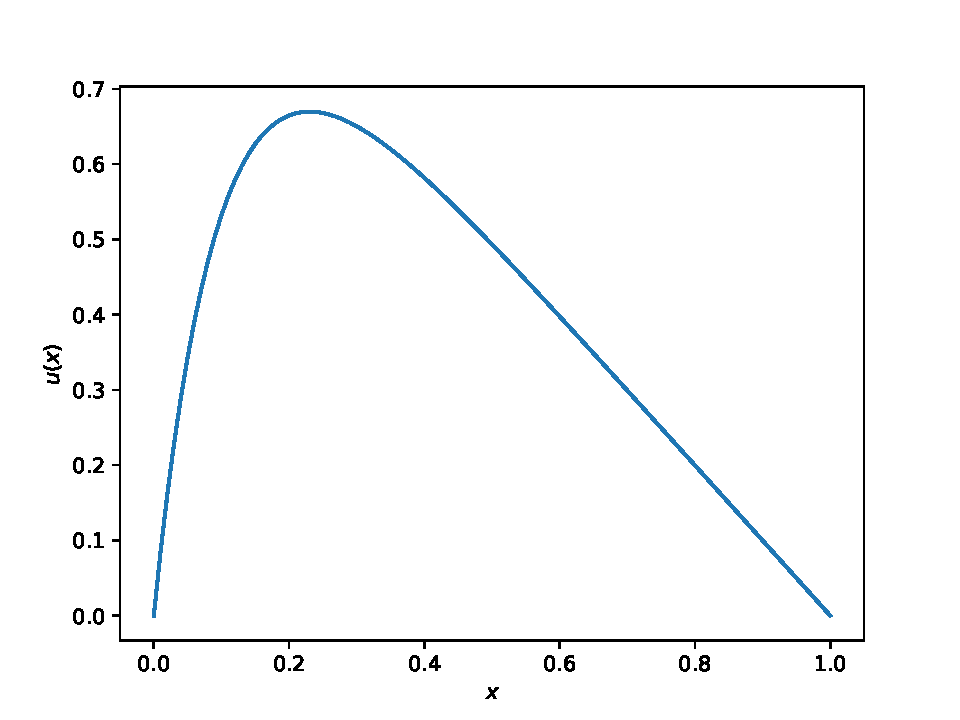
\includegraphics{/Users/alessiocanclini/FYS4150/project1/figures/x_u_plot.pdf}
  \caption{Plot of $u(x)$.}
  \label{tab:output_table}
\end{figure}

\section*{Problem 3}

\section*{Problem 4}

\section*{Problem 5}

\section*{Problem 6}

\section*{Problem 7}

\section*{Problem 8}

\section*{Problem 9}

\section*{Problem 10}
We write equations using the LaTeX \texttt{equation} (or \texttt{align}) environments. Here is an equation with numbering
\begin{equation}\label{eq:newton}
    \vb{F} = \dv{\vb{p}}{t},
\end{equation}
and here is one without numbering:
\begin{equation*}
\oint_C \vb{F}\cdot \dd \vb{r} = 0.
\end{equation*}
Sometimes it is useful to refer back to a previous equation, like we're demonstrating here for equation \ref{eq:newton}.

We can include figures using the \texttt{figure} environment. Whenever we include a figure or table, we \textit{must} make sure to actually refer to it in the main text, e.g.\ something like this: ``In figure \ref{fig:rel_err} we show \ldots''.
\begin{figure}%[h!]
    \centering %Centers the figure
    \includegraphics[scale=0.55]{} %Imports the figure.
    \caption{Write a descriptive caption here that explains the content of the figure. Note the font size for the axis labels and ticks --- the size should approximately match the document font size.}
    \label{fig:rel_err}
\end{figure}
Also, note the LaTeX code we used to get correct quotation marks in the previous sentence. (Simply using the \texttt{"} key on your keyboard will give the wrong result.) Figures should preferably be vector graphics (e.g.\ a \texttt{.pdf} file) rather than raster graphics (e.g.\ a \texttt{.png} file).

By the way, don't worry too much about where LaTeX decides to place your figures and tables --- LaTeX knows more than we do about proper document layout. As long as you label all your figures and tables and refer to them in the text, it's all good. Of course, in some cases it can be worth trying to force a specific placement, to avoid the figure/table appearing many pages away from the main text discussing it, but this isn't something you should spend time on until the very end of the writing process.


Next up is a table, created using the \texttt{table} and \texttt{tabular} environments. We refer to it by table \ref{tab:output_table}.
\begin{table}%[h!]
    \centering
    \begin{tabular}{c@{\hspace{1cm}} c}
        \hline
        Number of points & Output \\
        \hline
        10 &  0.3086\\
        100 &  0.2550\\
        \hline
    \end{tabular}\caption{Write a descriptive caption here, explaining the content of your table.}\label{tab:output_table}
\end{table}

Finally, we can list algorithms by using the \texttt{algorithm} environment, as demonstrated here for algorithm \ref{algo:midpoint_rule}.
\begin{algorithm}[H]
    \caption{Some algorithm}\label{algo:midpoint_rule}
    \begin{algorithmic}
        \State Some maths, e.g $f(x) = x^2$.  \Comment{Here's a comment}
        \For{$i = 0, 1, ..., n-1$}
        \State Do something here
        \EndFor
        \While{Some condition}
        \State Do something more here
        \EndWhile
        \State Maybe even some more math here, e.g $\int_0^1 f(x) \dd x$
    \end{algorithmic}
\end{algorithm}

\end{document}
